\section{Measuring the performance of the pipeline}\label{e2e}

Above results reflect the performance of the \ac{ASR} stage alone. To get some insight about the quality of alignments produced by the whole pipeline, a simple web application was implemented that highlights the aligned parts of the transcript as the audio file is being played. This is very useful for an informal review, because the subjective quality of the alignments can be examined interactively. However, this method is not very systematic and infeasible for larger amounts of test data. To get a clearer sense of how well the pipeline performs, steps were taken to run large numbers of previously unseen samples through the pipeline and measure the quality of the final product (the alignments). This section describes how this was done.

\subsection{The quality of alignments}

Assessing the quality of alignments is not trivial because there is often no reference alignment to compare to. Even if there is one, assessing the quality of an alignment is somewhat subjective because a different alignment does not necessarily need to be worse or better. Objectively quantifying the quality of a result is difficult for an alignment pipeline because there is a a massive number of theoretically possible alignments for each audio/text combination. We can however derive a few objective criteria that make up a good alignment:

\begin{enumerate}
	\item The aligned partial transcripts should not overlap each other
	\item The alignments should neither start nor end within word boundaries
	\item The aligned partial transcripts should cover as much of the original transcript as possible	
	\item The aligned partial transcripts should be at the correct position, i.e. they should cover the actually spoken text
\end{enumerate}

The first criterion is enforced by changing the type of algorithm used for sequence alignment from a local to a global alignment algorithm. The \textit{Smith-Waterman} algorithm was used in the \ac{LSA} stage in the IP8 project, which finds a local optimum for each transcript in isolation. The \ac{LSA} stage in this project uses global sequence alignment (\textit{Needle-Wunsch} algorithm), which finds an optimal alignment for all partial transcrips at once. 

The second criterion is ensured by adjusting some of the alignments so that they fall exactly on word boundaries. This is done by moving the alignment boundaries produced by the \textit{Needle-Wunsch} algorithm to the left or right, depending on which one is closer. Figure \ref{needle_wunsch_adjustment} shows an example.

\begin{figure}
	
\includegraphics[width=\linewidth]{./img/placeholder.png}
	\caption{Examples of how the alignment boundaries calculated by \textit{Needle-Wunsch} to the left or right}
	\label{needle_wunsch_adjustment}
\end{figure}

The remaining two criteria can be quantified with the following metrics (note the corellation\footnote{positive correlation: higher is better, negative correlation: lower is better}):

\begin{table}[!htbp]
	\centering
	\begin{tabular}{llll}
		\toprule
		\thead{criterion} & \thead{metric} & \thead{symbol} & \thead{correlation} \\
		\midrule
		1 & \makecell[l]{length of text in ground truth that is not aligned\\vs. total length of the ground truth} & $C$ & negative\\ \\ 	
		3 & \makecell[l]{average Levensthein similarity between the transcript\\and the text in the ground truth corresponding to its alignment} & $D$ & positive \\ 
		\bottomrule
	\end{tabular}
	\caption{Metrics to evaluate the quality of alignments}
	\label{LM_evaluation}
\end{table}

Because the first metric measures how much of the target transcript is covered by the alignments, it is similar to the Recall metric ($R$) usually used for classification tasks. The second metric measures how well the produced results match up with the underlying parts of the transcript and is therefore similar to Precision ($P$). Both metrics can hence be reduced to the \textit{F-score} ($F$):

\[ 
F = 2\cdot \frac{P\cdot R}{P+R}
 \]

Figure \ref{example_alignment} shows a constructed example of how the inferred partial transcripts (predictions) are aligned with the known full transcript (ground truth) of an audio/text sample.

\begin{figure}
	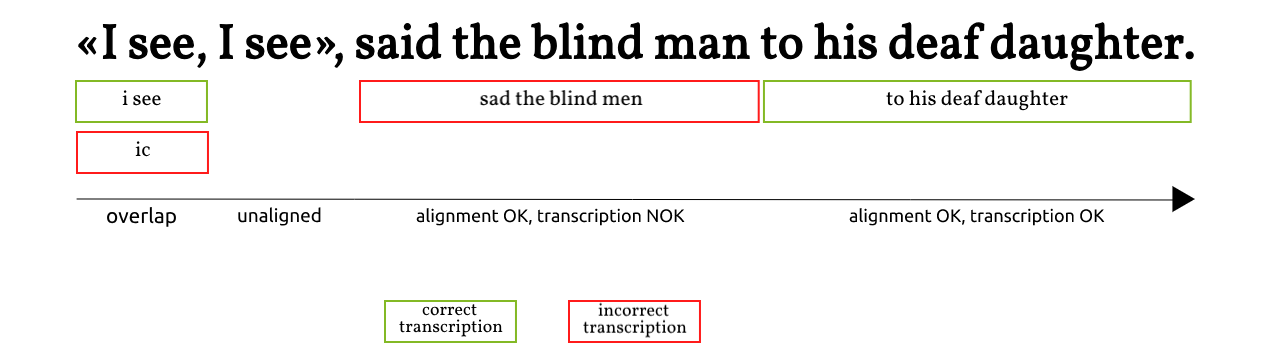
\includegraphics[width=\linewidth]{./img/example_alignment.png}
	\caption{Example for a partially correct alignment of parts of a sentence}
	\label{example_alignment}
\end{figure}

\subsection{Test and results}

The pipeline was evaluated on the test set of the \textit{LibriSpeech} corpus containing 87 audio/text samples. Each sample was run through the pipeline twice using different \ac{STT} models in the \ac{ASR} stage:

\begin{enumerate}
	\item Simplified Keras model: the dropout-regularized model trained on 1.000 minutes was used, because it had the lowest average \ac{LER} value on the validation data. Training was stopped early after 15 epochs to prevent overfitting. 
	\item Reference model: the pre-trained model downloaded from the project page of the Mozilla implementation\footnote{\url{https://github.com/mozilla/DeepSpeech\#getting-the-pre-trained-model}} was used
\end{enumerate}

Running the samples through both pipelines should help comparing the results produced by the first pipeline against a hypothetical optimum. Apart from the model used in the \ac{ASR} stage, all other stages in the pipeline were identical. The average values of $P$, $R$ and $F$ over all test samples was calculated for each pipeline. Figure \ref{pipeline_boxplot_ls_en} 

\begin{figure}
	
\includegraphics[width=\linewidth]{./img/placeholder.png}
	\caption{Average values of $P$, $R$ and $F$ for a pipeline using the simplified \ac{STT} model compared to a pipeline using a state of the art model}
	\label{pipeline_boxplot_ls_en}
\end{figure}
